\documentclass[11pt, letterpaper, oneside]{article}
\usepackage[utf8]{inputenc}

\usepackage[english]{babel}

\usepackage[
    %backend=biber,
    %style=alphabetic,
    citestyle=authoryear-icomp
    ]{biblatex}

\renewbibmacro{in:}{}
\addbibresource{MyLibrary.bib} %Imports bibliography file
\usepackage{graphicx}
\usepackage{geometry}
\usepackage{hyperref}
\usepackage{relsize}
\usepackage{amsmath}
\usepackage{csquotes}
\usepackage{inputenc}
\usepackage{caption}
\usepackage{subcaption}
\geometry{letterpaper, margin=1in}

\title{Project Proposal: "Representation Learning with Self-teaching Conditional Generative Adversarial Networks"}
\author{Itsuki Ogihara} %\thanks{TBD}}
\date{}

%\theoremstyle{theorem}
\newtheorem{theorem}{Theorem}[section]

\begin{document}
\maketitle

\begin{abstract}
In recent years, the field of Representation Learning has been receiving great attention due to its attractive premise, and some of the recent results have demonstrated its potential. \cite{chen_isolating_nodate}\cite{higgins_-vae_2017}. One of the most popular approaches that has been attracting much attention in recent years is generative adversarial Networks, or GANs (\cite{goodfellow_generative_2014}), which in general is used in an unsupervised setting by having two agents compete with one another. Despite its apparent success with impressive results, other recent studies have shown its limitations and argued that such unsupervised representation learning is fundamentally infeasible \cite{locatello_challenging_2019}. From this perspective, we take a step back and revisit semi-supervised GANs architectures\cite{mirza_conditional_nodate}, \cite{chen_self-supervised_2019}, and further investigate their potential as a basis to learn representation as a set of conditions. Guided by the principle outlined by \cite{bengio_representation_2014}, we seek to capture the distinctness of the data in a 'disentangled' form. In this light, we demonstrate how such representation as sets of conditions can be constructed and empirically test its capacity for both discrete and continuous variables as well as their combinations. Furthermore, we test for the disentangled-ness of such representation by testing individual conditions separately. Finally we propose and test a pipeline for training and constructing representations using conditional GANs architecture.
\end{abstract}

\section{Introduction}
\paragraph{}
The main idea behind the representation leaning is intuitive. Informally, the goal of representation learning is to find useful transformations $x \rightarrow r(x) = y$ that “make it easier to extract useful information when building classifiers or other predictors” \cite{bengio_representation_2014}. Many models used in representation learning recently are generative models. Intuitively, if a model is capable of 'generating' some output based on some information presented to it, it may be reasonable to assume that the model has learnt some sort of representational quality of the given data, and therefore may be used for representation learning as well. One of the most recent developments in this field is the use of GANs. It has shown remarkable capacity to learn features and manipulate and synthesize them into a desired output, which lends itself as a natural candidate for representation learning. There have been successful attempts which demonstrated that its intermediate stage can be shown as an evidence of feature segmentation. Notably, \cite{radford_unsupervised_2016} has proposed a method that visualizes the filters learnt by GANs and empirically shows that specific filters have learned to draw specific objects using a technique called guided back-propagation, which was originally proposed by \cite{springenberg_striving_2015}. Despite its successful result, since this method utilizes derivatives of the error as an insight to what is being modified in the model during the training, it is not immediately clear how we are able to use this information with respect to representation learning.
\paragraph{}
In representation learning, we strive for a more fundamental, universal form of abstraction. Such representation would immediately find itself useful in many applications; for example, it is easy to see how such representation would be helpful when transfer leaning is involved. If a model is able to extract some features that are transferable or mutually understandable between different tasks or spaces, ideally such representation should be invariant to the space it originates in but more universal. One way of towards achieving this goal is to seek for 'disentangled' representation as defined by \cite{bengio_representation_2014}. Although there is no formal definition of 'disentanglement' in the context of representation leaning has been established (\cite{locatello_challenging_2019}), yet, general consensus is that such representation should be able to separate the distinct, informative factors of variations in the data (\cite{bengio_representation_2014}). Despite the need and highly desirable nature of such representation, the progress that has been seen in this field has been either application specific or trivial.
\paragraph{}
To highlight the lack of more general representation learning methods, \cite{locatello_challenging_2019} has recently challenged some of the claims that are made in the field of representation learning by theoretically demonstrating that the unsupervised learning of \textit{disentangled} representations is fundamentally impossible without inductive biases on both the models and the data. Also, they have run empirical experiments using the proposed algorithms and observed that, while the different methods successfully enforce properties “encouraged” by the corresponding losses, well-disentangled models seemingly cannot be identified without supervision. Further more, they also noted that increased disentanglement does not necessarily lead to a decreased sample complexity for the downstream tasks, which cast an existential doubt on such representation.     
\paragraph{}
From this perspective, a pursuit for a \textit{good} representation in a completely unsupervised manner seems infeasible as it is done in the most recent research. Hence, in this paper, we take a step back from the unsupervised learning, and reexamine a more traditional supervised approach. Namely, we will investigate the conditional-GANs \cite{mirza_conditional_nodate} and view it as an approach to generate disentangled features. Conditional-GANs was originally motivated from the observation that original GANs' generates outputs based on random noise had no constraints on them. This characteristic made the model's output unconditional and therefore unpredictable. \cite{mirza_conditional_nodate} proposed a simple way to introduce some conditions on the input space and empirically demonstrated that specific conditioning resulted in targeted outputs that are reflective of imposed conditions. Though its empirical results were promising, the study was limited in scope in terms of the conditions that were tested and demanded further investigation. More specifically, to what extent a condition can be imposed or whether multiple conditions can be placed simultaneously was not part of the original study. In this paper, we propose several testing schemes to gain further insight in this area and to test more complex conditions of a higher order, such as interactions can be observed. Specifically, we propose to test the model's ability to respond to the following conditioning:

\begin{itemize}
\item \textbf{Discrete condition} We test if we can manipulate the type of output generated. We will test whether a model can learn to produce specific class of output. This is partially a repeat of what has been demonstrated by \cite{mirza_conditional_nodate}. We extend to this by imposing different type of discrete condition.

\item \textbf{Continuous condition} We test if we can control the degree of manipulation of distinct features individually. For example, rotation and volume (size of characters) can be imposed with a varying degree. We hypothesise that this will be a harder task to learn than the discrete condition as outlined above. This comes from the intuition that, for discrete conditions, the learning is done though memorizing characteristics for each class; however in continuous conditioning, such memorization may be harder to achieve since not all intermediate samples are supplied in the form of input data.  

\item \textbf{Higher order condition} We test if we can control several aspects of features simultaneously. We test combinations of both discrete and continuous conditions. Specifically, we test the combination of two discrete conditions, both discrete and continuous, and two continuous conditions.

\item \textbf{Disentangled condition} We test if the conditions can be constructed as disentangled components. Since we seek to find 'useful' representation, we hope this representation to be \textit{disentangled.}, that is, each conditions are imposed \textit{compositionally}. This experiment will be different from the higher order condition in the sense that we are testing the models' ability to produce outputs as a composition of distinct features and we hope to be able to control them separately. This is in part related to the field of 'compositionality' in machine learning, and was largely motivated by \cite{hupkes_compositionality_2020}. Here, we are interested in finding if the model has learnt to produce features in a compositional manner.

\end{itemize}
\paragraph{}
The main goal of this study is not an improvement over the other proposed representation leaning models but to offer an alternative approach to finding useful representation in general. By \textit{useful}, we mean that to be 'disentangled' and good characterization. Again, this is motivated by the finding by \cite{locatello_challenging_2019}, that the idea of deriving a portable representation in an unsupervised manner as in many of the recent researches have shown, might not be as useful as it claims. Alternatively, we propose to incorporate \textit{conditioning} as an auxiliary representation that can supplement the existing representation learning methods. And by automating the training process to derive such representation by way of self-supervising, we demonstrate how this form of learning can be incorporated into existing methods. Although the proposed approach may not necessarily result in a \textit{compact} representation, it may yet be beneficial to a wide range of downstream tasks.
\paragraph{}
In the following section \ref{RelatedWork}, we review a few key relevant works and the theoretical background needed for our study. In section \ref{SScGANs}, we will explain the experiments in detail as well as the models that are used in the experiment. In section \ref{Results_Discussion}, we will present and discuss the result followed by the proposed training pipeline. In the last section \ref{Summary}

\section{Related Works} \label{RelatedWork}
\subsection{Representation Learning}
 \cite{bengio_representation_2014} solidified the concept of 'representation learning' as "learning representations of the data that make it easier to extract useful information when building classifiers or other predictors. Then naturally, the next question to ask is what constitutes a "good representation". We have seen great success in generating \textit{self-representation} e.g. unsupervised autoendoders \cite{vincent_stacked_nodate},\cite{rifai_contractive_nodate} and manifold learning \cite{rifai_contractive_nodate} and other dimension reduction techniques. Yet, many of them are focused on \textit{self-representation} as they are interpretable only by their own creators. To take this beyond \textit{self-representation}, \cite{bengio_representation_2014} identified three key qualities needed for such representation, i.e. they should be 'distributed', invariant', and 'disentangled'.  Distributed representation means that the representation needs to be expressive, so that it can capture a reasonably-sized learned representation, which in turn can capture a large number of configurations. Invariance refers to the level of abstraction, as more abstract representation should be invariant to local changes of the input. The hardest and arguably the most controversial is the notion of \textit{disentanglement}, which roughly refers to its ability to \textit{disentangle} the input space so as to segregate distinct aspects of the given data. This is discussed further in the subsequent section. %Note that \cite{bengio_representation_2014} also suggests that this process has to be done at least in a semi-supervised manner in order for this to be of practical use. 
 
\subsubsection{Disentanglement}
From the beginning of the pursuit for representation learning, it has been noted that the key factor of successful representation leaning lays in its ability to learn features that are distinct and \textit{controllable} independently of others.
When we face a complex data, often we find a intricate web of interacting features that affects the outcome, which in turn makes it increasingly more difficult to control or understand the correlation between the input and the output. 
This is related but different from the definition of invariance in that invariance, by definition, has reduced sensitivity in the direction of invariance. The goal of invariance extraction is to build features that are insensitive to variation in the data that are uninformative to the task at hand. On the other hand, disentanglement implies a certain degree of information loss/retention. More specifically, disentanglement is 'to disentangle as many factors as possible, discarding as little information about the data as is practical' \cite{bengio_representation_2014} 

Such representation is important as it may lead to a more interpretable model and shed some light onto the the inner workings of the models in general. Also, having access to such information should help ease the task downstream. Furthermore, increased disentanglement may lead to to a decreased sample complexity for the downstream tasks. We argue that the notion of \textit{disentanglement} is related to the compositionality of a model as outlined by \cite{hupkes_compositionality_2020}, that is, if a model is learning compositionally, it indicates that each component of the representations should be independent of one another. 

\subsection{Generative Adversarial Networks (GANs)}
In recent years, generative adversarial networks (GANs) have gained in popularity and have been shown to produce impressive results. It has also been deployed in many representation learning settings as mentioned in the earlier section.  Since it was originally proposed by \cite{goodfellow_generative_2014},  numerous variations were proposed that are shown to improve its performance in terms of computation and its output quality. GANs are, in general, a class of \textit{unsupervised} generative models that involve two models within itself, a \textit{generator} and a \textit{discriminator} which works \textit{adversarial} to one another such that, together, it plays a min-max game in order to improve the overall performance of the model. More formally, it can be expressed as following:
\begin{equation} \label{eu_eqn000}
 \min_{G}  \max_{D} V(C, D) = \mathbf{E}_{x \sim P_{data(x)}}[log D(x)] + \mathbf{E}_{z \sim P_z(z)}[log {(1-D(G(z))}]
\end{equation}
where $P_{data}$ is the true data distribution and $P_z$ is the distribution generated by the generator. To learn a generator distribution over the data x, the generator generates a function that takes $p_z(z)$, a 'noise' as a prior and maps to the data space $G(z)$ and the discriminator $D(x)$ is a function that represents the probability that x came from the data or from the generator generated distribution $G(x)$. We optimize both the generator and discriminator in a min-max game setting, i.e., we maximize the Equation 1 with respect to the parameters and then we try to minimize it and repeat until the desired level of output is generated.  This framework is very flexible and its generative nature has inspired many researchers to adopt this technique in representation learning as it renders itself quite naturally into its framework.

\subsubsection{Deep Convolutional GANs (DCGANs)} 
One of such attempts is Deep Convolutional GANs (DCGANs) \cite{radford_unsupervised_2016}, which incorporate convolutional neural networks (CNN) within the generator architecture. %Though this approach was tried prior to DCGANs, the training process proved to be unstable. 
DCGANs propose a set of guidelines for constructing Deep Convolutional GANs, which included removal of fully connected layers, use of batch normalization, use of Relu activation, use of strided convolutions (for discriminator) and fractional-strided convolutions (for generator) instead of using pooling layers. 
They empirically demonstrated their performance in classification task. In addition, by visualizing the intermediate state using guided back-propagation as proposed by \cite{springenberg_striving_2015}, it showed that the model is capable to learning hierarchy of features, i.e. it was shown to learn the features that are of most interest. Though the evidence was convincing, in the context of representation learning, the use of such derivative-based representation is not immediately useful for our purpose and need alternative form of extracting information.

% \subsection{Information Maximizing Generative Adversarial Nets (InfoGANs)}
% Built on the idea of DCGANs, \cite{chen_infogan_2016} proposed the use of mutual information, an information-theoretic regularization term as a part of objective function to be optimized. More formally, let $c$ denote a latent code, given any $x \sim P_G(x)$ where $G$ is the generator, we want $P_G(c|x)$ to have a small entropy, that is, the information in the latent code $c$ should not be lost in the generation process though $G$, which can be expressed as
% \[ \min{G} \max{D} V_I(D, G) = V(D, G) - \lambda I(c; G(z, c))  \]
% where $z$ denotes the noise that is passed to the generator along with $c$. \cite{chen_infogan_2016} demonstrated that this approach can be used to extract disentangled representations such as writing style, shape and other notable features completely unsupervised using MNIST, CelebA, and a 3D chair bench marking data set.   

\subsection{Limitation of unsupervised representation learning}
Despite that some impressive developments are being made, \cite{locatello_challenging_2019} has challenged its claim, the idea that real-world data is generated by a few explanatory factors of variation which can be recovered by unsupervised learning algorithms. \cite{locatello_challenging_2019} has theoretically demonstrated that the unsupervised learning of disentangled representation is fundamentally impossible without inductive bias on both models and the data. The basis for this claim hinges on the following theorem:
\begin{theorem}
For $d > 1$, let $z \sim P$ denote any distribution which admits a density p(z) = $\prod ^d_{i=1}p(z)$. Then, there exist as infinite family of objective functions $f: supp(z) \rightarrow supp(z)$ s.t. $\frac{\delta f_i(u)}{\delta u_j} \ne 0$ almost everywhere for all $i$ and $j$ and $P(z <= u) = P(f(z) < u)$ for all $u \in supp(z).$
\end{theorem}

This theorem basically shows that if $z$ and $f(z)$ have the same marginal distribution,  $z$ and $f(z)$ cannot be completely disentangled. However, \cite{locatello_challenging_2019} notes that while the above theorem shows that unsupervised disentanglement learning is fundamentally impossible, this does not exclude all the efforts in practice, since some generative models may have a certain structure that could be exploited by having suitable inductive biases. In the context representation learning with GANs, the inductive biases are on the choice of architecture, cost functions, and regularization mechanisms used during the training, as well as the data set itself. 
Though the finding may not appear too surprising, it does however remind us to consider a more careful approach to the analysis of representation learning. 

\subsection{Semi-supervised GANs}
In this light, we take a step back from the completely unsupervised GANs and re-examine the semi-supervised approaches and reassess its potential and possible applications in representation learning. More concretely, we view semi-supervised representation learning as a guided alternative to a fully unsupervised one, which can learn the specific features we are interested in via explicit conditions.

\subsubsection{Conditional GANs (cGANs)}
Early on in GANs development, \cite{mirza_conditional_nodate} demonstrated a simple method to achieve a certain degree of control over the output by inserting additional constraints on the inputs. The idea is to condition both the generator and discriminator using some extra information $y$. In this context $y$ can be any kind of auxiliary information that can be useful for downstream tasks such as class labels. With this modification, the objective function now becomes

\begin{equation} 
 \min_{G} \max_{D} V(C, D) = \mathbf{E}_{x \sim P_{data(x)}}[log D(x|y)] + \mathbf{E}_{z \sim P_z(z)}[log (1-D(G(z|y))]
\end{equation}

\cite{mirza_conditional_nodate} empirically showed that such conditioning can lead to some control over the generated outputs which had otherwise been completely random. For example, the output of unconditional GANs can be very \textit{accurate} yet, we had no way to tell what type of output it would generate.   

\subsubsection{Self-Supervised GANs}
The immediate drawback of conditional GANs is that they require labeled data, which can be hard and expensive to obtain at times. To address this issue, a more recent study by \cite{chen_self-supervised_2019} proposed a novel technique for training GANs in a self-supervised manner. This is achieved by introducing the use of self-supervised loss to the discriminator. This was demonstrated by the imposition of 'rotation' condition on a image. Consider an image generation task where generator is provided with a original image and an additional information that encodes a degree of rotation (i.e $0^{\circ}, 90^{\circ}, 180^{\circ}, 270^{\circ}$) and this information is also shared with the discriminator. This allows the discriminator to not be punished for the handicap placed by the rotation of the original image. More formally, the loss function for the generator and the discriminator now becomes,
\begin{equation}
L_G = -V(C, D) -\alpha \mathbf{E}_{x \sim P_G } \mathbf{E}_{r \sim R}[log Q_D(R = r|x^r)]
\end{equation}
\begin{equation}
L_D = V(C, D) -\beta \mathbf{E}_{x \sim P_{data} } \mathbf{E}_{r \sim R}[log Q_D(R = r|x^r)]
\end{equation}

where $V(G, D)$ is the same value function from \equationautorefname{1}, $r \in \mathbb{R}$ is a rotation imposed on the input data. $x^r$ denoted the input with the selected input imposed on them. $Q( r \in \mathbb{R} | x^r )$ denotes the discriminator's predictive distribution over the rotation of the sample provided. \cite{chen_self-supervised_2019} empirically demonstrated their proposed model attains similar performance to the one that's attained using fully conditional GANs.
  
\section{Self-supervised conditional GANs for representation learning} \label{SScGANs}
\paragraph{}
The conditional GANs and self-supervised GANs framework provide a simple yet solid foundation for deriving a representation that can be used for controlling single simple aspect of the output. It can be interpreted as an extraction of a specific aspect of the input data, which is an essential feature of disentangled representation. The results demonstrated by \cite{chen_self-supervised_2019} were a clear proof of concept. However, the range of their experiment was limited in scope. It tested its ability on a single conditioning factor, the rotation. Furthermore, the rotation values that were presented to the model were limited to a very small number of options. By design, the model had only 4 rotation variations to choose from in terms of the input and the output, which made the rotation condition essentially a discrete variable, though the rotation in general is not considered to be a discrete condition but rather a continuous one.
\paragraph{}
In this paper, we take this idea further and test if this method can be applied to a different set of conditions and of higher order, by which we mean the additive combination of multiple conditions as well as interaction of conditions. We will employ a MNIST digit data set of hand written digits from 0 to 9, each 28 x 28 in size. The color was muted to gray scale only. This dataset is widely used including \cite{chen_self-supervised_2019}, which allows a direct comparison of our result to their out predecessors. 

\subsection{Single Condition}
First, we are interested in finding and extracting a wider set of features respectively. We test if we can disentangle a feature for discrete conditions as well as continuous conditions. Specifically, we are interested in optimizing the following:

\begin{equation} \label{eu_eqn0}
L_G = -V(C, D) -\alpha \mathbf{E}_{x \sim P_G } \mathbf{E}_{c \sim C}[log Q_D(C = c|x^c)]
\end{equation}
\begin{equation} \label{eu_eqn01}
L_D = V(C, D) -\beta \mathbf{E}_{x \sim P_{data} } \mathbf{E}_{c \sim C}[log Q_D(C = c|x^c)]
\end{equation}
where $c \sim C$ denoting target condition from a condition class $C$, $c \in C$, $\alpha, \beta $ are the hyper parameters for associated terms respectively.
\paragraph{}
We then seek to condition the input on the following features:
\begin{itemize}
    \item \textbf{Classification}(Discrete condition): Condition on the class to generate class specific output, i.e. we specify the target class for the output.  \newline
    Here class refers to the single digit number represented by the image i.e. (0, 1,...9) which is presented to the model as a one-hot coded equivalent. At the test time, we specify the outputs by conditioning the input to one of each digits from $N(0,9)$ No modification to the original data was done for this experiment. 
    
    \item \textbf{Color} (Discrete condition): Condition on the color (black on white vs while on black).  \newline
    This will be presented to the model as a binary indicator, i.e., 0 indicating white letter against black background, 1 indicating black letter against while background. The training samples' colors were randomly inverted $50\%$ of the time so that half of the training data consists of the original color and the other half consists of the inverted version. 
    
    \item \textbf{Rotation} (Continuous condition): Condition on the rotation of the image. \newline
    This is almost the same experiment conducted by \cite{chen_self-supervised_2019}, except that we have provided a wider range of conditions. Instead of limiting the rotation angles to the multiple of $90^{\circ}$ we have used smaller increments, i.e. incremented by $18^\circ$. The intention of this experiment is to replicate \cite{chen_self-supervised_2019} and use this condition later in combination with other conditions. The rotation condition is presented to the model as a single number between -1 and 1 indicating the degree of rotation. s.t. $ r \in \mathbb{R}$ and  $|r| \leq 1$. To test if the model has learned this condition as a continuous value as opposed to simply memorizing the input by just associating certain conditions with a desired output, we test the model by proposing conditions that were unseen during the training. This is equivalent to the zero-shot learning in the literature. If the model has indeed learnt to see the condition as continuous we expect the model to generate appropriate output for the given condition. Also, since we are interested in conditioning on rotation and rotation only at this time, we use only a subset of training data for one of the digits only. (We arbitrarily chose 5.)
    
    \item \textbf{Size} (Continuous condition) : Condition of the size of the object drawn. We vary the size of object drawn within the frame in proportion to the original. \newline
    The condition was imposed in 5 distinct increments. This number was chosen so as to allow visual inspection. Any smaller increments were determined to be too hard to be visually distinguished. Same as with the rotation condition, we used only the subset of the training data for this part of experiment. (We arbitrarily chose digit 2.) This condition was presented to the model as a number between 0 and 1, 0 indicating a small, 1 indicating a large body within a frame. s.t $ t \in \mathbb{R}$ and  $ 0 \leq t \leq 1$. Again, to test for the continuity of the condition, we test the model via zero-shot leaning i.e. present an input that were either in between the conditions that were \textit{seen} during the training, as well as numbers that are out of range of what was seen during the training. 
\end{itemize}

\subsection{Multi-level Condition}
We also test to see if more than one condition can be imposed simultaneously to induce more complex target outputs. We hypothesise that this task will be substantially harder than the previous experiment. In order to compare the quality of the image being generated, we use the accuracy metric from the discriminator. We assume that an output that yields the equal level of accuracy by the discriminator would be of equal quality. We are also interested in if and/or how the conditions may interact. To this end, the objective functions now becomes,

\begin{equation} 
L_G = -V(C, D) -\alpha \mathbf{E}_{x \sim P_G } \mathbf{E}_{c_1  \sim C_1}\mathbf{E}_{c_2  \sim C_2}[log Q_D(C_1 = c_1, C_2= c_2|x^{(c_1, c_2)})]
\end{equation}
\begin{equation}
L_D = V(C, D) -\beta \mathbf{E}_{x \sim P_{data} } \mathbf{E}_{c_1 \sim C_1}\mathbf{E}_{c_2  \sim C_2}[log Q_D(C_1 = c_1, C_2= c_2|x^{(c_1, c_2)})]
\end{equation}
Here, the expected value is based on the number of samples in the training set for the particular condition being considered.
We then consider the following combination of conditions. A few modified examples are shown in \figureautorefname{1}.
\begin{itemize}
    \item \textbf{Classification + Color} (Discrete + Discrete condition): Condition on the class to generate AND the color simultaneously. \newline
    This experiment is almost the same as the Color experiment, but this time both the digit and color conditions were imposed. As before, both conditions were presented in a binary format. Also, as in the Color experiment, roughly half of the training set was converted to be color-inverted. At the testing time, we specify the output via two levels of conditions. The quality of the output is then assessed by the 'accuracy' metric from the discriminator. 
    
    \item \textbf{Classification + Rotation} (Discrete + Continuous condition): Condition on the class AND the rotation of the image simultaneously. \newline
    For this experiment, each training data is rotated at 10 predetermined rotation angles incremented by $36^{\circ}$ $x={0, 36, 72, ..., 360}$ then this information along with the digit label was passed to the discriminator as its input. Note that this modification to the input practically resulted in an increase of the training data by a factor of 10, that is, the number of rotations per sample. As with the earlier rotation experiment, we test the continuity of the condition via zero-shot learning. In this context, this means presenting a model with rotation angles that are either in between the increments or some number from out of range. Again, we use the accuracy metrics from the discriminator as the quality indicator for comparison.
    
    \item \textbf{Rotation + Size} (Continuous + Continuous condition): Condition of the rotation AND the size of the object drawn. \newline
    For this experiment, each sample was subjugated to two continuous conditions. For training this model, we modified each sample in the training set to be rotated at 5 predetermined rotation angles incremented by $18^{\circ}$ $x={0, 45, 90, 135, 180}$ and 5 predetermined sizing increments as outlined in the sizing experiment. As a result, the training set size practically increased by a factor of 25. As before, we test the continuity of the conditions via zero-shot learning. In this context, this means presenting a model with both rotation angles and sizing conditions that are either in between the increments or some number from out of range. Again, we use the accuracy metrics from the discriminator as the quality indicator for comparison.
    
\end{itemize}

% \begin{figure}[h!]
%     \centering
%     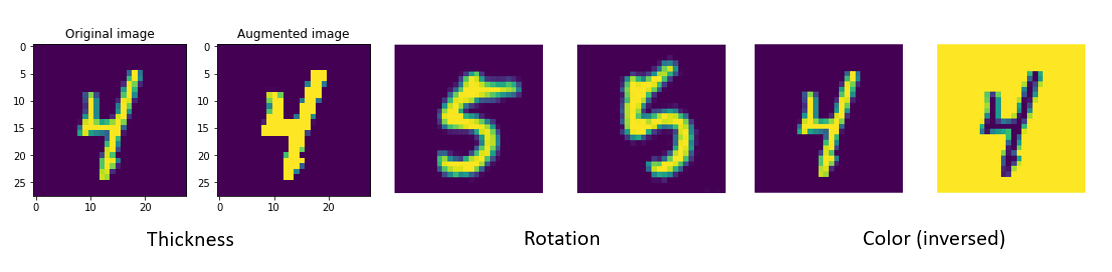
\includegraphics[width = 5in]{ImageAugSample.png}
%     \caption{Conditioned Image Examples}
%     \label{fig:classification}
% \end{figure}

\subsubsection{Disentangled Conditioning}
In this section, we investigate whether the learned representation is \textit{disentangled}. As our goal is to seek a 'good' representation of data, it is critical that the representation learnt is indeed dedicated to a specific feature, i.e., we would like the representation as a means to gain control of distinct aspects of outputs respectively. \newline
This concept of disentanglement is related to the discourse around 'compositionality' in neural networks. If the goal is to design a machine that is capable of learning concepts in a compositional manner, one would expect that it can generate outputs that are 'composed' of distinct components. If the alternative is true, a model that is trained using two conditions would not be capable of generating output with only one condition imposed. That is, the model simply associated a certain combination of conditions with the desired output. To test whether our model has learnt to impose multiple conditions respectively, we further exploit the experiments for the multi-condition with additional constraints:

\begin{itemize}
    \item \textbf{Classification + Color} (Discrete + Discrete condition): In order to test if only one of the discrete conditions can be imposed one at a time, we replace one of the conditions with random noise that does not resemble any previously seen during the training.\newline
    \begin{equation*}
    Example
        [0, 1, 0, 0, 0, 0, 0, 0, 0, 0] \longrightarrow [0.79, 0.45, 0.02, 0.81, 0.85, 0.32, 0.46, 0.90, 0.57, 0.75]
    \end{equation*}
    Specifically, first, to test if only class condition can be imposed, we provide the generator usual binary labels for the class and random noise from $N(0,1)$ instead of the binary color specification. We conduct the same to test for conditioning only on the color by replacing the binary classification.
    
    \item \textbf{Classification + Rotation} (Discrete + Continuous condition): In this setting, we are interested in testing 1) if only a discrete condition can be imposed 2) if only one continuous condition can be imposed at a time. \newline
    For this purpose, for 1), we test the models trained under Discrete + Continuous condition by providing the model with an input that is outside of what has been seen during the training. \newline
    For 2) we simply replace the class condition with random number as in the previous experiment.

    \item \textbf{Rotation + Size} (Continuous + Continuous condition): In this setting, we are interested in testing if one of the continuous conditions can be imposed at a time. \newline
    Using the same scheme as before, we present the generator with one of the conditions replaced with random number that is outside of range seen during the training. 

All the above testing schemes embrace the principle of zero-shot learning: the main idea is to present a model that it has not trained with which in turn will force the model to generate a unique output based on a composition of conditions that is learnt to impose, not from simply resorting to memorized desired output. 

\end{itemize} 

\section{Self-teaching pipeline for training Conditional GANs}
\paragraph{}
To facilitate the training and testing scheme presented above, we demonstrate a training pipeline that streamlines the process of self-generating samples and distributes the information to both the generator and the discriminator. 
\begin{itemize}
    \item Step 1: Teacher($T$) selects condition(s) $c$ for training samples ($x$) 
    \item Step 2: Teacher generates conditioned training sample ($T(x, c) = x^c$) for Discriminator, and noise vector for generator and passes them along with the condition(s) ($(z, c)$)
    \item Step 3: Generator generates outputs based on the input from T ($G(z, c) = z^c$)
    \item Step 4: Discriminator evaluates $z^c$ and $x^c$ (Discriminator loss)
    \item Step 5: Discriminator sends feedback to the generator (Generator loss)
\end{itemize} 
We implemented the above in a mini-batch so each iteration consists of multiple batch operation to go through; each training data then was repeated over many iterations until certain accuracy was achieved. We monitor both the discriminator loss and generator loss. We also monitor the classification accuracy of discriminator and use this as a proxy for the quality of the image generated by the generator. This process is illustrated in Figure \ref{fig:Self-teaching GANs}  

\begin{figure}[h!] \label{Teacher}
    \centering
    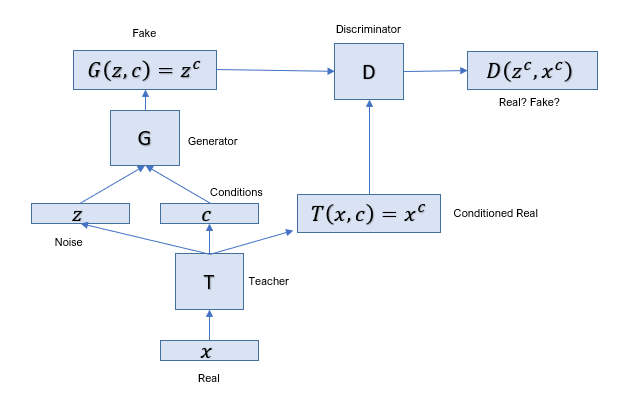
\includegraphics[width=10cm]{SelfTeachingGANsArchitecture.png}
    \caption{Self-teaching GANs Architecture}
    \label{fig:Self-teaching GANs}
\end{figure}

\paragraph{}
This architecture is more complex than \cite{chen_self-supervised_2019} in that it automates the condition selection and conditioned input generation process. Also the range of conditions that can be imposed is more flexible and not limited to be discrete, but includes continuous ones. Moreover, under this scheme it is possible to impose multiple conditions simultaneously. In our experiment, we compile condition vectors with a simple concatenation method then passed to the generator as its input. However, this can be modified for different applications. We note that since the conditioned samples are generated online during the training, it eliminates the need for extra storage to keep the samples which can be inflated by the number of conditions. For a high-dimension data like image, that may be an added benefit. However, we recognize that the only method would likely be to slow down the training process substantially compared to the offline implementation. 

\subsubsection{Neural Networks}
For the network structure of generators and discriminator, we follow the guidelines proposed in DCGANs(\cite{radford_unsupervised_2016})  with a minor modification to fit our data. For the generator, we will have 4 blocks of networks stacked in a sequential manner, each consisting of one convolutional layer, followed by batch normalization and LeakyRelu nonlinear activation, except for the last block where we simply use the output from the convolutional layer. In each convolutional layer we will have 4x4 filter with stride of 2, fixed for all the convolutional layers. For the generator, the architecture is almost the same as for the discriminator except for that we use transposed convolution in place of convolution and in the output layer, we will use tanh activation. This is illustrated in \figureautorefname{3} and \figureautorefname{4}. 
A notable feature of these networks is that they use no fully connected or pooling layers as recommended by \cite{radford_unsupervised_2016}. For training, we used a mini batch size of 32 that was kept the same for all the experiments conducted. 

% \begin{figure}[ht]
%     \centering
%     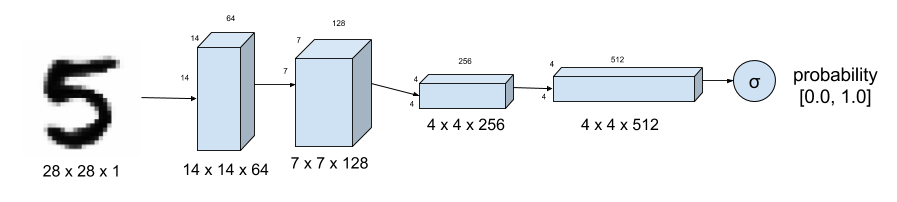
\includegraphics[width=10cm]{discriminatorArch.png}
%     \caption{Discriminator Architecture}
%     \label{fig:disc}
% \end{figure}
% \begin{figure}[htbp]
%     \centering
%     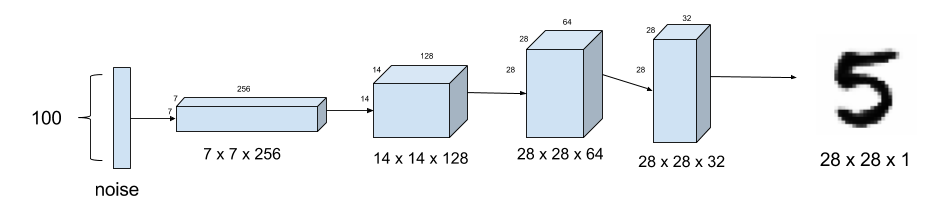
\includegraphics[width=10cm]{generatorArch.png}
%     \caption{Generator Architecture}
%     \label{fig:gen}
% \end{figure}
%\subsection{Summary}

% \begin{figure}
% %\centering
% \begin{minipage}{.5\textwidth}
%   \centering
%   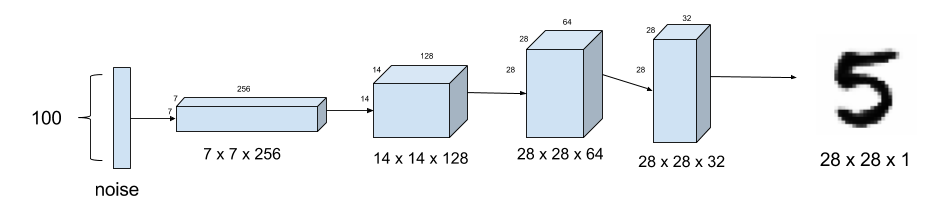
\includegraphics[width=5cm]{generatorArch.png}
%   \captionof{Figure}{Generator Architecture}
%   \label{fig:test1}
% \end{minipage}%
% \begin{minipage}{.45\textwidth}
%   \centering
%   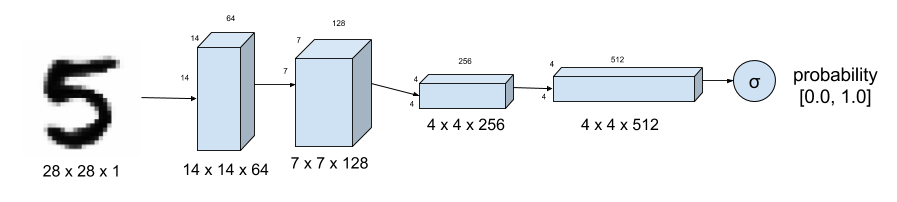
\includegraphics[width= 5cm]{discriminatorArch.png}
%   \captionof{Figure}{Discriminator Architecture}
%   \label{fig:test2}
% \end{minipage}
% \end{figure}

\begin{figure}
    \begin{subfigure}{.5\textwidth}
      \centering
      % include first image
      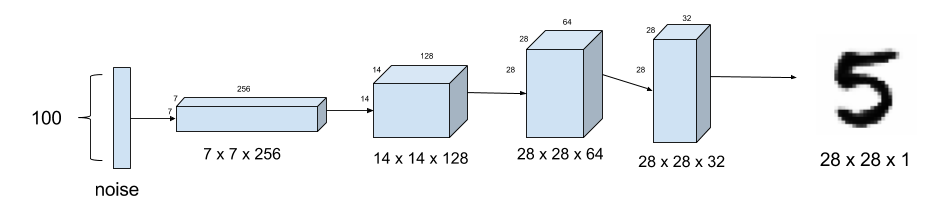
\includegraphics[width=1\linewidth]{generatorArch.png}  
      \caption{Generator}
      \label{fig:sub-first}
    \end{subfigure}
    \begin{subfigure}{.5\textwidth}
      \centering
      % include second image
      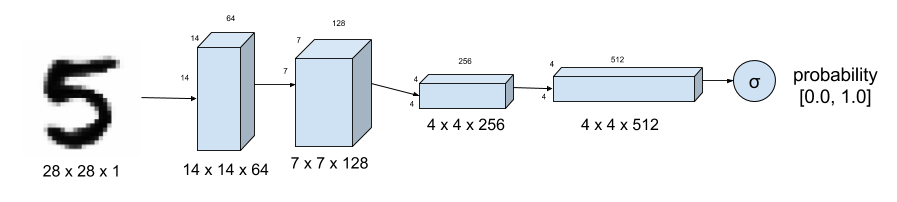
\includegraphics[width=1\linewidth]{discriminatorArch.png}  
      \caption{Discriminator}
      \label{fig:sub-second}
    \end{subfigure}

\caption{Network Architecture}
\label{fig:fig}
\end{figure}
  

\section{Results and Discussion} \label{Results_Discussion}

\subsection{Single Condition}

\begin{figure}
    \begin{subfigure}{.5\textwidth}
      \centering
      % include first image
      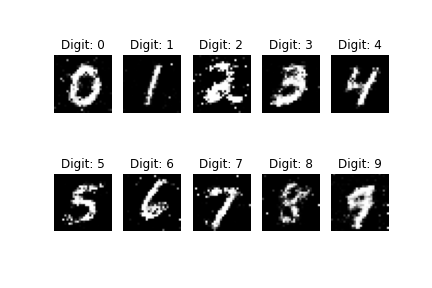
\includegraphics[width=1\linewidth]{classification.png}  
      \caption{Classification}
      \label{fig:sub-first}
    \end{subfigure}
    \begin{subfigure}{.5\textwidth}
      \centering
      % include second image
      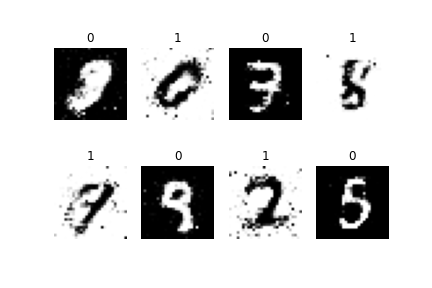
\includegraphics[width=1\linewidth]{inv.png}  
      \caption{Color}
      \label{fig:sub-second}
    \end{subfigure}

\newline

    \begin{subfigure}{.5\textwidth}
      \centering
      % include third image
      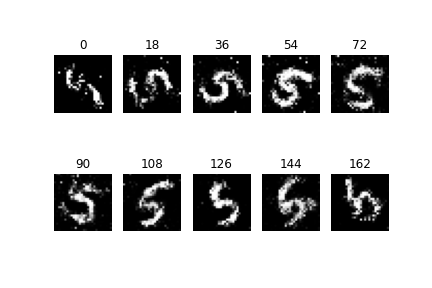
\includegraphics[width=1\linewidth]{rotation.png}  
      \caption{Rotation}
      \label{fig:sub-third}
    \end{subfigure}
    \begin{subfigure}{.5\textwidth}
      \centering
      % include fourth image
      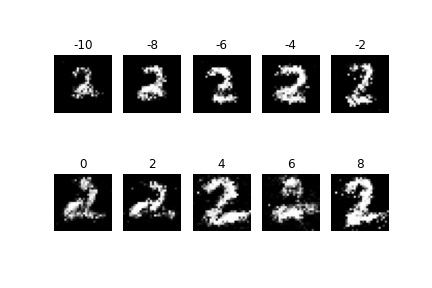
\includegraphics[width=1\linewidth]{size.png}
      \caption{Size}
      \label{fig:sub-fourth}
    \end{subfigure}
\caption{Single Condition}
\label{fig:fig}
\end{figure}
  

When faced with a single condition, most of the 4 cases achieved high accuracy of $\sim 60$\% within a relatively small number of iterations. (As a reminder, the accuracy metrics used here refer to the accuracy of the discriminator, therefore a score close to $\sim$ 50\% is considered to be the perfect score where the discriminator is unable to properly distinguish the real sample from the training set and the output from the generator.) However, we observe that there was a noticeable difference between discrete and continuous conditions in the number of iterations required to reach the same level of accuracy. In Classification and Color experiment, it took about 5000 iterations to achieve 60\% accuracy, while it took about 10,000 for Rotation, 15000 for Size conditions, respectively.   
Also, we observed that when the generator was presented with zero-shot samples, the output matched the expected samples fairly well. And this was true for both Rotation and Size experiments. This result indicates that the model did not simply memorize the target output but rather it has learned to generate the output based on the conditions given. However, we also noted that in a zero-shot setting, i.e., when the condition provided was far out of range that is seen during the training, the output failed to reflect such extreme value. In other words, it did not extrapolate. For example, in Size experiment, when presented with conditions that are too small or too large, the output generated seemed to converge to the smallest or largest sample that was seen during the training. 

\subsection{Multiple Conditions}
% \begin{itemize}
%      \item \textbf{Classification + Color} (Discrete + Discrete condition):  
    
%     \item \textbf{Classification + Rotation} (Discrete + Continuous condition): 
    
%     \item \textbf{Rotation + Size} (Continuous + Continuous condition):    
% \end{itemize}

\begin{figure}
    \begin{subfigure}{.5\textwidth}
      \centering
      % include first image
      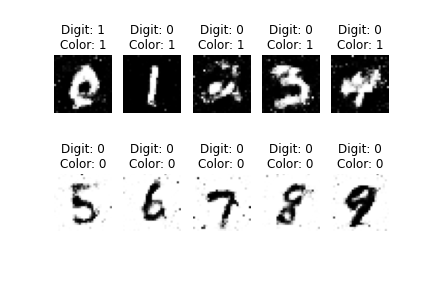
\includegraphics[width=1\linewidth]{dig_inv.png}  
      \caption{Classification + Color}
      \label{fig:sub-first}
    \end{subfigure}
    \begin{subfigure}{.5\textwidth}
      \centering
      % include second image
      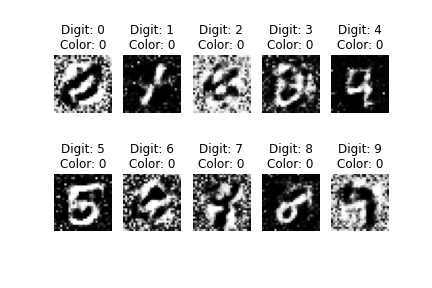
\includegraphics[width=1\linewidth]{digit_no_color.png}  
      \caption{Classification + Color (ZS)}
      \label{fig:sub-second}
    \end{subfigure}

%\newline

    \begin{subfigure}{.5\textwidth}
      \centering
      % include first image
      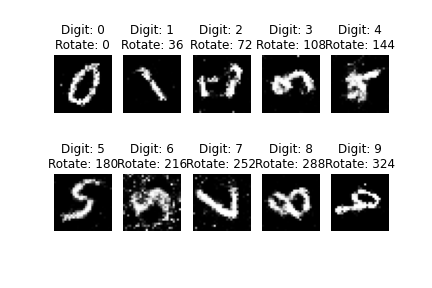
\includegraphics[width=1\linewidth]{digit_rotate.png}  
      \caption{Classification + Rotation}
      \label{fig:sub-first}
    \end{subfigure}
    \begin{subfigure}{.5\textwidth}
      \centering
      % include second image
      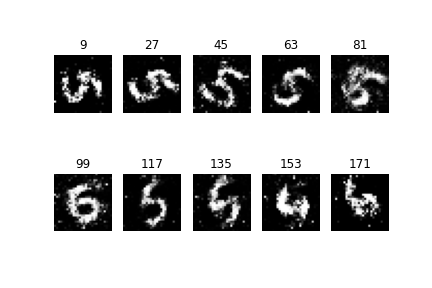
\includegraphics[width=1\linewidth]{rotation_ZSL.png}  
      \caption{Classification + Rotation (ZS)}
      \label{fig:sub-second}
    \end{subfigure}

%\newline

    \begin{subfigure}{.5\textwidth}
      \centering
      % include third image
      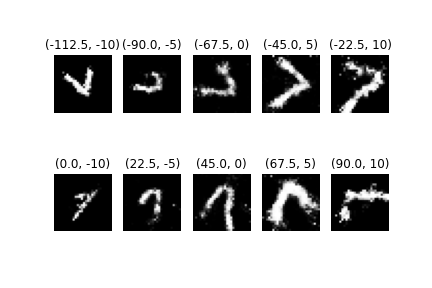
\includegraphics[width=1\linewidth]{rotation_size.png}  
      \caption{Rotation + Size}
      \label{fig:sub-third}
    \end{subfigure}
    \begin{subfigure}{.5\textwidth}
      \centering
      % include fourth image
      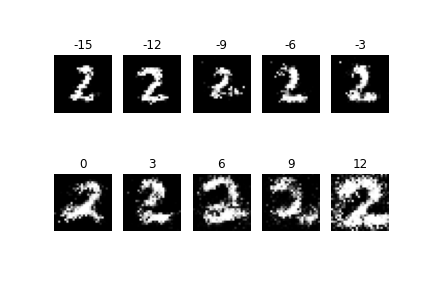
\includegraphics[width=1\linewidth]{size_ZSL.png}
      \caption{Rotation + Size (ZS)}
      \label{fig:sub-fourth}
    \end{subfigure}
    
\caption{Multiple Conditions}
\label{fig:fig}
\end{figure}

In a Multi-condition setting, overall all of the experiments required many more iterations to reach the same level of accuracy compared to the single condition. Although this result was expected, we noticed that the iterations requirement growth was not simply linear in the number of conditions imposed. For example, for Classification + Color experiment, it took about 20000 iterations to reach 60\% accuracy where it took about 5000 each when imposed separately, which indicates that complexity may increase exponentially in the number of conditions. 
For Classification + Rotation, the difference in training time requirement was even starker. It took about 200,000 iterations to achieve the same level of accuracy of $\sim$ 60\%. Compared to Classification and Rotation experiments which took about 5000 and 10000 iterations respectively, it took roughly 20 times more iterations. This result differs from the previous experiment but the gap is far larger.  We suspect that this may be related to the number of conditions seen during the training. The number of 'combinations' of conditions increased from 10 to 10*10 = 100 compared to the single condition experiment. We also tested the model in a ZSL setting for the continuous condition. The result was similar to what we have found in the single condition setting. For intermediate values (within the range of the train data), the output was almost as it is expected to produce, i.e., it generated outputs that are in 'between' samples that are indeed seen during the training. For out-of-range values, the output was similar to the closest sample from the training set but failed to generate unique or original output solely based on the given condition. 
For Rotation + Size, the iteration required to reach the threshold accuracy of 60\% was around 20,000, which was substantially less than what was observed in Classification + Rotation. In the single condition setting Rotation and Size, each took about 10,000 iterations, hence the growth rate is close to linear in the number of conditions. Con

\subsection{Disentanglement}
% \begin{itemize}
%      \item \textbf{Classification + Color} (Discrete + Discrete condition):  
    
%     \item \textbf{Classification + Rotation} (Discrete + Continuous condition): 
    
%     \item \textbf{Rotation + Size} (Continuous + Continuous condition): 
% \end{itemize}

\begin{figure}
    \begin{subfigure}{.5\textwidth}
      \centering
      % include first image
      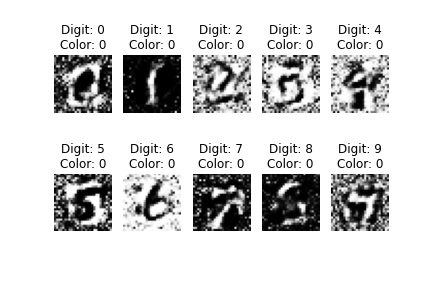
\includegraphics[width=1\linewidth]{Digit_Color_ZSL.png}  
      \caption{Classification + Random Color}
      \label{fig:sub-first}
    \end{subfigure}
    \begin{subfigure}{.5\textwidth}
      \centering
      % include second image
      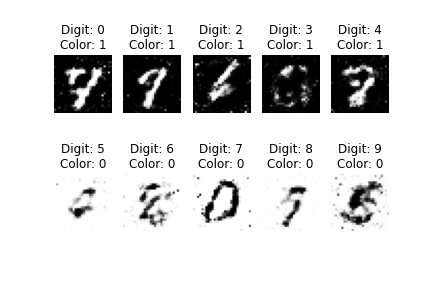
\includegraphics[width=1\linewidth]{Digit_ZSJ_Color.png}  
      \caption{Random Classification + Color}
      \label{fig:sub-second}
    \end{subfigure}

%\newline

    \begin{subfigure}{.5\textwidth}
      \centering
      % include first image
      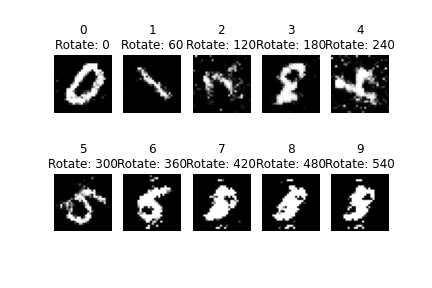
\includegraphics[width=1\linewidth]{Digit_RotateZSL.png}  
      \caption{Classification + Rotation}
      \label{fig:sub-first}
    \end{subfigure}
    \begin{subfigure}{.5\textwidth}
      \centering
      % include second image
      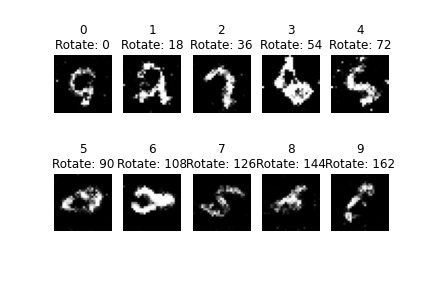
\includegraphics[width=1\linewidth]{DigitZSL_Rotate.png}  
      \caption{Classification + Rotation (ZS)}
      \label{fig:sub-second}
    \end{subfigure}

%\newline

    \begin{subfigure}{.5\textwidth}
      \centering
      % include third image
      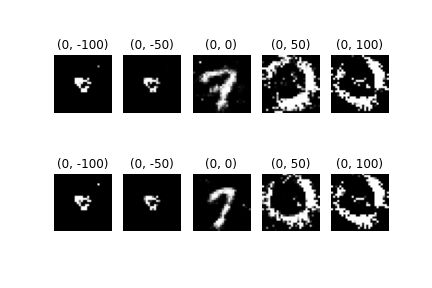
\includegraphics[width=1\linewidth]{rotate_sizeZSL1.png}  
      \caption{Rotation + Random Size}
      \label{fig:sub-third}
    \end{subfigure}
    \begin{subfigure}{.5\textwidth}
      \centering
      % include fourth image
      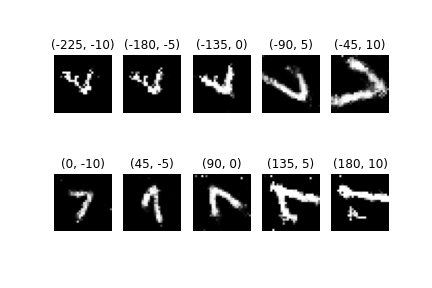
\includegraphics[width=1\linewidth]{rotateZSL_size.png}
      \caption{Random Rotation + Size}
      \label{fig:sub-fourth}
    \end{subfigure}
    
\caption{Disentanglement}
\label{fig:fig}
\end{figure}

To test whether the model has learned disentangled features, we tested the pre-trained model from the previous experiments by semi-conditioning the input. We fed the generator with one of the conditions replaced with a random number or out-of-range values. The purpose of this set of experiments is to test whether a model has learned to distinguish operations and is capable of applying each independently. This is an important aspect of 'disentangled' learning. If the model is capable of such learning, we expect the model to be able to impose one condition at a time; however, if the model has simply memorized each 'combination' of conditions, it would not be capable of separating the two and therefore would not be able to produce a singularly conditioned output if the model was trained under multi-condition setting. 

In Classification + Color (discrete, discrete) experiment, we observed that when a Color condition was replaced with unseen random noise, the output still reflected the specified Classification, while the Color of the output became rather random and in many cases gray or uneven reflecting the random nature of the Color condition provided. This observation is particularly interesting in that the output was a unique and original generation and did not resemble any of training samples. In turn, when the Classification conditions were replaced with random noise, output generated random numbers with no coherent pattern, while perfectly reflecting the Color conditions imposed on them. This result again implies that the model is capable of imposing distinct operations separately, indicating its compositional learning ability. 

In Classification + Rotation (discrete, continuous) experiment, we observed that when the Classification condition was replaced with random numbers, the digits represented became random with no coherent pattern, reflecting the random nature of the specification, while still managing to reflect the rotation condition imposed. In turn, in testing the Rotation condition in a ZSL setting, we observed that if the rotation specification was interpolation, i.e., within the range seen in the training set, the outputs reflected both the specified conditions as expected from the previous experiment. On the other hand, when the rotation condition was extrapolation, we observed that the model was less capable of specifying the Class condition when the Rotation conditions shifted further away from the training set. When the rotation range was far beyond the familiar range, the digits representation became increasingly ambiguous. For some extreme value, the output has shown a clear sign of mode collapse, i.e., it generates the same outputs for all combinations of conditions. This result can be seen as a sign that the model did not learn the two conditions separately, but rather learnt them in tandem and is therefore unable to separate and treat them as distinct concepts. This result contradicts the earlier finding in Classification + Color (discrete, discrete) experiment.   

In Rotation + Size (continuous, continuous) experiment, we observed the similar tendency that the model was capable of generating expected outputs by interpolating the training set. Even then the exact combination of the conditions was not directly seen during the training. This was the case for both rotation and size condition. For extrapolation, when the size condition was extrapolated, output no longer retained the original shape as expected. The image no longer resembled the digits in the training sample while faithfully reflecting the size condition, again showing signs of mode collapse. Similarly, when the rotation condition was extrapolated, the output suffered from mode collapse. And the output resembled the samples with the closest pair of conditions seen during the training.

\section{Summary and Future Works} \label{Summary}
We demonstrated how GANs may be used in a self-supervised setting to learn representation that is disentangled using training involving conditioning. We proposed a general pipeline and architecture for training such a model. Specifically, we empirically tested its ability to learn discrete conditions, continuous conditions, as well as their combinations. We further investigated its ability to learn compositionally as a way to demonstrate disentangled. We observed that the model we proposed was capable of learning continuous conditions, though it was limited to interpolation. When the model was tasked with extrapolation, all the outputs collapsed to the closest match from the training set. We also observed that the model was capable of learning disentangled features when the conditions were either both discrete or both continuous. This ability diminished when the task involved both discrete and continuous conditions simultaneously.   
This paper only tested up to two conditions to be imposed together. But future work should extend to idea to include more layers of conditions, different types of conditions, as well as their combinations. Also, we did not include other forms of 'conditioning' other than what has been proposed in this paper, though there are other techniques that exist. It would be interesting to see how different conditioning methods interact with its ability to learn salient features.


\printbibliography

\end{document}